%versi 3 (18-12-2016)
\chapter{Hasil Pengujian Eksperimental}
\label{lamp:C}

%terdapat 2 cara untuk memasukkan kode program
% 1. menggunakan perintah \lstinputlisting (kode program ditempatkan di folder yang sama dengan file ini)
% 2. menggunakan environment lstlisting (kode program dituliskan di dalam file ini)
% Perhatikan contoh yang diberikan!!
%
% untuk keduanya, ada parameter yang harus diisi:
% - language: bahasa dari kode program (pilihan: Java, C, C++, PHP, Matlab, C#, HTML, R, Python, SQL, dll)
% - caption: nama file dari kode program yang akan ditampilkan di dokumen akhir
%
% Perhatian: Abaikan warning tentang textasteriskcentered!!
%
\section{Hasil Pengujian Eksperimental Mahasiswa}
\begin{figure}[H]
	\centering
	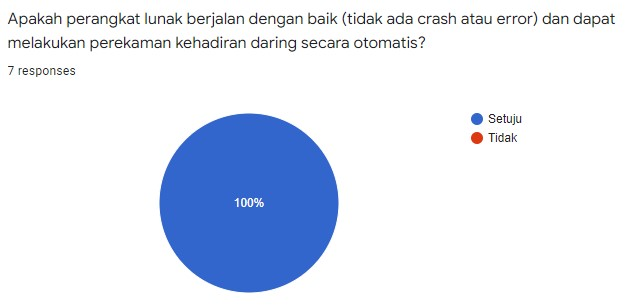
\includegraphics[scale=0.75]{Gambar/SurveiMahasiswa1.jpg}
	\label{}
	\caption{Jawaban responden(Mahasiswa) untuk pertanyaan pertama.}
\end{figure}

\begin{figure}[H]
	\centering
	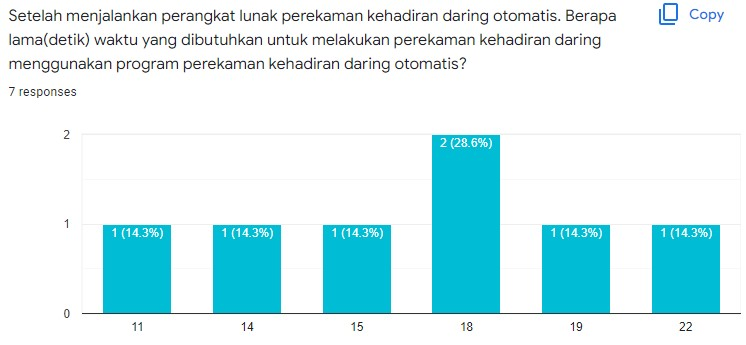
\includegraphics[scale=0.75]{Gambar/SurveiMahasiswa2.jpg}
	\label{}
	\caption{Jawaban responden(Mahasiswa) untuk pertanyaan kedua.}
\end{figure}
	
\begin{figure}[H]
	\centering
	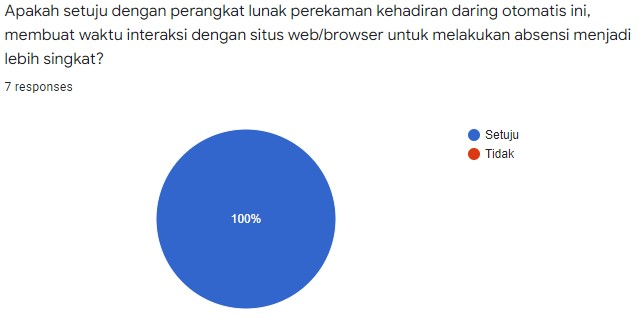
\includegraphics[scale=0.75]{Gambar/SurveiMahasiswa3.jpg}
	\label{}
	\caption{Jawaban responden(Mahasiswa) untuk pertanyaan ketiga.}
\end{figure}
	
\begin{figure}[H]
	\centering
	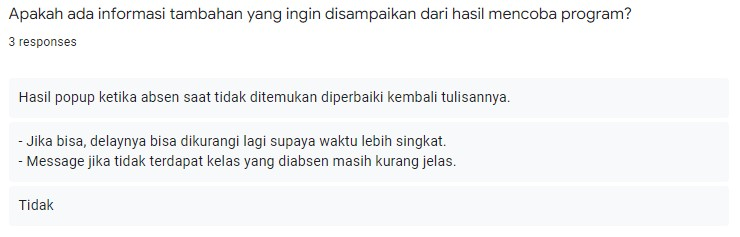
\includegraphics[scale=0.75]{Gambar/SurveiMahasiswa4.jpg}
	\label{}
	\caption{Jawaban responden(Mahasiswa) untuk pertanyaan keempat.}
\end{figure}

	
\section{Hasil Pengujian Eksperimental Dosen}
\begin{figure}[H]
	\centering
	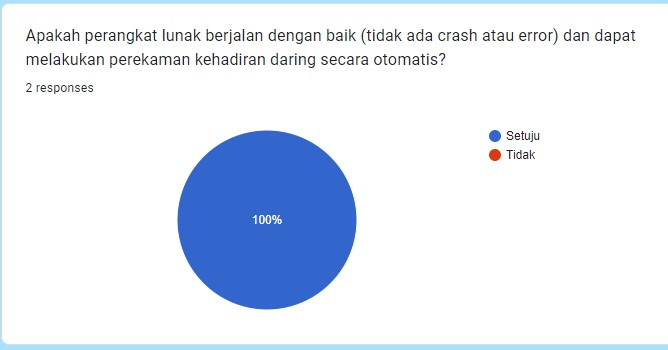
\includegraphics[scale=0.75]{Gambar/SurveiDosen1.jpg}
	\label{}
	\caption{Jawaban responden(Dosen) untuk pertanyaan pertama.}
\end{figure}
	
\begin{figure}[H]
	\centering
	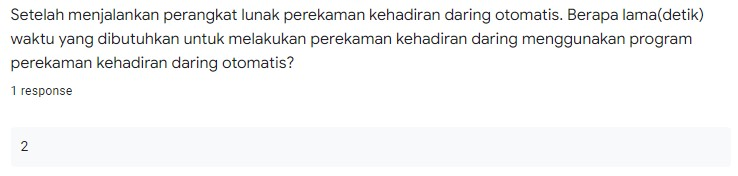
\includegraphics[scale=0.75]{Gambar/SurveiDosen2.jpg}
	\label{}
	\caption{Jawaban responden(Dosen) untuk pertanyaan kedua.}
\end{figure}

\begin{figure}[H]
	\centering
	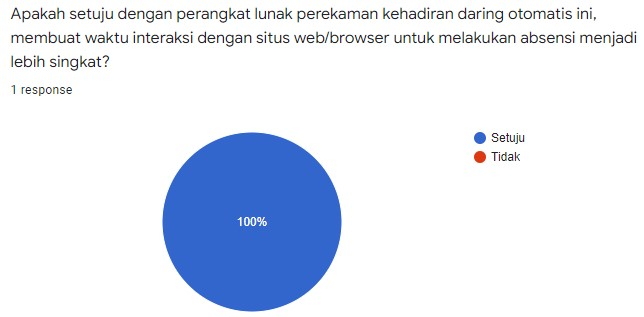
\includegraphics[scale=0.75]{Gambar/SurveiDosen3.jpg}
	\label{}
	\caption{Jawaban responden(Dosen) untuk pertanyaan ketiga.}
\end{figure}	

\begin{figure}[H]
	\centering
	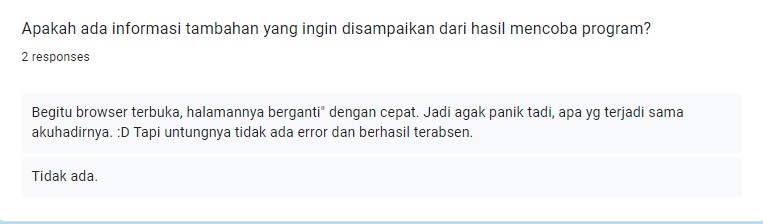
\includegraphics[scale=0.75]{Gambar/SurveiDosen4.jpg}
	\label{}
	\caption{Jawaban responden(Dosen) untuk pertanyaan keempat.}
\end{figure}	